% ==============================================================================
% Section 6: Integrated Derivative Hedging Efficiency
% ==============================================================================

\section{Integrated Derivative Hedging Efficiency}
\label{sec:hedging}

In Section~\ref{sec:var_modeling}, we established that an institutional investor holding \textbf{1 market lot} ($1,725$ shares of ITC at $S_0 = \text{\rupee}285.00$, $V_0 = \text{\rupee}4,91,625.00$) faces an empirical 10-day $99\%$ Historical Simulation $\VaR$ of \textbf{\rupee 61,487.02} ($12.51\%$ of capital), corresponding to an implied terminal spot floor of $S_{T, \VaR} = \text{\rupee}249.36$ per share.

To neutralize this tail risk, we evaluate three non-linear derivative structures:
\begin{enumerate}[leftmargin=1.8em, noitemsep]
    \item \textbf{ATM Protective Put ($K = \text{\rupee}285$):} Purchases pure downside insurance ($P_{\text{ATM}} = \text{\rupee}8.86$). The total premium cost across the lot is $1,725 \times \text{\rupee}8.86 = \text{\textbf{\rupee 15,283.50}}$ ($3.11\%$ of capital). For any terminal price $S_T < \text{\rupee}285.00$, the equity drawdown is entirely offset by the put payoff, strictly capping maximum capital loss at the upfront premium paid (\rupee 15,283.50). This achieves a \textbf{75.14\% VaR reduction}.
    \item \textbf{OTM Protective Put ($K = \text{\rupee}280$):} Procures lower-cost insurance ($P_{\text{OTM}} = \text{\rupee}6.82$, total outlay \rupee 11,764.50). The investor absorbs the first \rupee 5.00 deductible per share; below \rupee 280, all losses are insulated. Maximum portfolio loss is capped at $1,725 \times (5.00 + 6.82) = \text{\textbf{\rupee 20,389.50}}$, achieving a \textbf{66.84\% VaR reduction}.
    \item \textbf{Zero-Cost Collar Strategy (Put \rupee 280 / Call \rupee 295):} Finances the protective \rupee 280 put ($P = \text{\rupee}6.82$) by writing an OTM \rupee 295 covered call ($C = \text{\rupee}4.32$). The net upfront debit is only:
    \begin{equation}
    \text{Net Debit} = 6.82 - 4.32 = \text{\textbf{\rupee 2.50 per share}} \quad (\text{Total Outlay } = \text{\textbf{\rupee 4,312.50}})
    \end{equation}
    Downside loss is capped at \rupee 7.50/share (\rupee 12,937.50 per lot), while upside gains are capped above \rupee 295.00 at \rupee 7.50/share (+\rupee 12,937.50). This yields the highest tail risk insulation (\textbf{+78.96\% VaR reduction}).
\end{enumerate}

\begin{figure}[htbp]
\centering
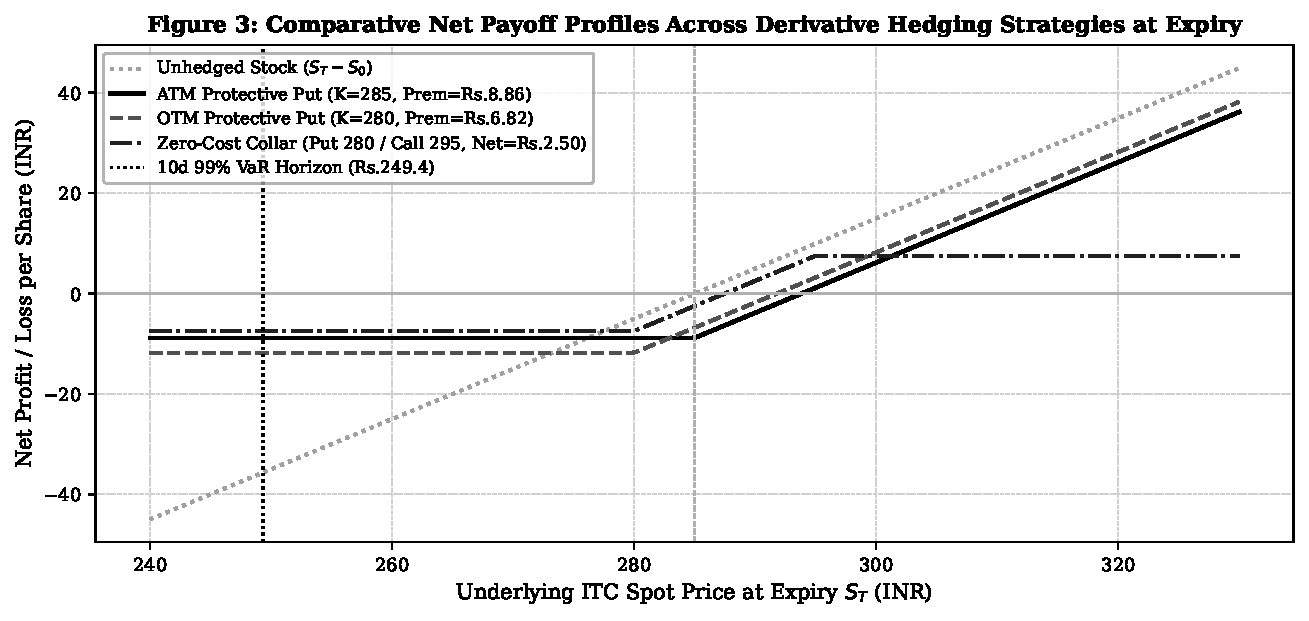
\includegraphics[width=0.96\linewidth]{figures/fig3_hedging_payoffs.pdf}
\caption{Comparative Net Payoff Profiles Across Derivative Hedging Strategies at Expiry}
\label{fig:hedging_payoffs}
\vspace{2pt}
\begin{minipage}{0.96\linewidth}
\footnotesize\textbf{Note:} Expiry profit/loss per share across terminal spot prices $S_T \in [\text{\rupee}240, \text{\rupee}330]$. Strategies: Unhedged Stock (dotted gray), ATM Protective Put (solid black), OTM Protective Put (dashed dark gray), and Zero-Cost Collar (dash-dot black). Vertical line indicates the 10-day $99\%$ $\VaR$ horizon ($S_{T, \VaR} = \text{\rupee}249.36$).
\end{minipage}
\end{figure}

Table~\ref{tab:hedging_summary} summarizes the comparative efficiency metrics across all four positions.

\begin{table}[htbp]
\centering
\small
\caption{Derivative Hedging Efficiency Matrix for 1 Lot of ITC ($1,725$ Shares, $V_0 = \text{\rupee}4,91,625$)}
\label{tab:hedging_summary}
\begin{tabularx}{\linewidth}{Xrrrr}
\toprule
\textbf{Quantitative Risk Metric} & \textbf{Unhedged Stock} & \textbf{ATM Put (285)} & \textbf{OTM Put (280)} & \textbf{Collar (280/295)} \\
\midrule
Position Architecture & $1,725$ Shares & Stock + Put 285 & Stock + Put 280 & Stock + P280 $-$ C295 \\
Upfront Cash Cost & \rupee 0.00 & \rupee 15,283.50 & \rupee 11,764.50 & \rupee 4,312.50 \\
Upfront Cost (\% of $V_0$) & $0.00\%$ & $3.11\%$ & $2.39\%$ & $0.88\%$ \\
Breakeven Expiry Price & \rupee 285.00 & \rupee 293.86 & \rupee 291.82 & \rupee 287.50 \\
Maximum Capital Loss ($1$ Lot) & $-\text{\rupee}4,91,625.00$ & $-\text{\rupee}15,283.50$ & $-\text{\rupee}20,389.50$ & $-\text{\rupee}12,937.50$ \\
Maximum Upside Potential & Unlimited & Unlimited & Unlimited & $+\text{\rupee}12,937.50$ (at 295) \\
\textbf{Loss at 10d 99\% VaR Horizon} & \textbf{-\rupee 61,487.02} & \textbf{-\rupee 15,283.50} & \textbf{-\rupee 20,389.50} & \textbf{-\rupee 12,937.50} \\
\textbf{Tail Risk Reduction (\%)} & \textbf{0.00\%} & \textbf{+75.14\%} & \textbf{+66.84\%} & \textbf{+78.96\%} \\
\bottomrule
\end{tabularx}
\end{table}

\begin{empiricalbox}{Hedging Efficiency and Execution Realities}{hedging_efficiency}
While dynamic delta replication ($\Delta_{\Pi} = 0$) requires continuous rebalancing that incurs high transaction costs and Securities Transaction Tax (STT) on the NSE, static option structures provide robust insurance against discontinuous overnight gap shocks. The \textbf{Zero-Cost Collar} provides the optimal risk-adjusted structure for institutional managers, cutting capital loss at the $99\%$ $\VaR$ horizon by \textbf{$78.96\%$} at a negligible cash drag of \rupee 4,312.50 ($0.88\%$ of portfolio value).
\end{empiricalbox}
